%laden der Präambel mit Latexbefehlen/-klassen
% !TeX encoding = UTF-8
% !TeX spellcheck = de_DE

%Dokumentklasse, Spracheinstellung, Schriften
\documentclass[a1paper,portrait]{baposter}
\usepackage[ngerman]{babel}
\usepackage[utf8]{inputenc}
\usepackage{arev}
\usepackage[T1]{fontenc}

%Mathe, Symbole, Einheitendarstellung, Chemie
\usepackage{amsmath}
\usepackage{amsxtra}
\usepackage{eurosym}
\usepackage{siunitx}  
\sisetup{locale=DE}
\usepackage[version=4]{mhchem}

%Typographie
\usepackage[auto]{microtype}

%Einbindung von Bildern, Tabellen, pdf-Seiten, Quellcode
\usepackage{booktabs}
\usepackage{multirow}
\usepackage{paralist}

%Darstellung der Literaturangaben
\usepackage[
backend=biber,
style=science,
citestyle=numeric-comp,
sorting=none,
maxbibnames=1,
firstinits=true
]{biblatex}

\bibliography{literatur/refs}
\setlength\bibitemsep{2.5pt}

%Definition der Farben
\definecolor{standardfontcolor}{RGB}{0,0,0} 
\definecolor{bordercol}{RGB}{113,113,113}
\definecolor{headercol1}{RGB}{255,255,255}
\definecolor{headercol2}{RGB}{113,113,113}
\definecolor{headerfontcol}{RGB}{0,0,0}
\definecolor{boxcolor}{RGB}{255,255,255}

\begin{document}
	\typeout{Poster rendering started}
	
\background{
	\begin{tikzpicture}[remember picture,overlay]%
	\draw (current page.north west)+(-2em,2em) node[anchor=north west]
	{\includegraphics[height=1.1\textheight]{figures/background}};
	\end{tikzpicture}
}

\color{standardfontcolor}

\begin{poster}{
		grid=false,
		columns=2,
		%colspacing=length
		headerheight=0.125\textheight,
		eyecatcher=false, 
		borderColor=bordercol,
		headerColorOne=headercol1,
		headerColorTwo=headercol2,
		headerFontColor=headerfontcol,
		% Only simple background color used, no shading, so boxColorTwo isn't necessary
		boxColorOne=boxcolor,
		headershape=roundedright,
		headerfont=\sffamily\bfseries\Large,
		textborder=rectangle,
		headerborder=open,
		boxshade=plain,
		background=none
%		background=user
	}
	%%% Eye Cacther %%%%%%%%%%%%%%%%%%%%%%%%%%%%%%%%%%%%%%%%%%%%%%%%%%%%%%%%%%%%%%%
	{
		Eye Catcher, empty if option eyecatcher=false - unused
	}
%----------------------------------------------------------------------------------------
%	TITLE AND AUTHOR NAME
%----------------------------------------------------------------------------------------
%
{
	\textsf %Sans Serif
	{FPGA-Accelerated Network IDS with RISC-V Co-Processor Integration}
}
{\sf\vspace{0.5em}\\
	Pinky*, Brain und Jane Doe
	\vspace{0.1em}\\
	\small{Technische Universität Berlin, Fakultät III, Vertiefendes Rechnerpraktikum zur Energietechnik
	\vspace{0.2em}\\
	* pinky@campus.tu-berlin.de}
}
% University/lab logo
{
\includegraphics[height=3cm]{bilder/logo/logo-gruppe-1.pdf}} 
%
%
\headerbox{Aufgabenstellung}{name=einleitung,column=0,row=0,span=2}{
Vorlage für die Erstellung eines Posters. Es wird die Klasse baposter verwendet. In der entsprechenden Dokumentation finden sich Hinweise zur Gestaltung. Die Vorlage bietet ein einfaches Layout, dass zur Bearbeitung der Aufgabenstellung ausreichend sein sollte. Die Einbindung verschiedener Elemente ist beispielhaft gezeigt.

Hier könnte die Einleitung stehen, also Motivation, Ziel der Arbeit, Aufgabenstellung, etc.

Literaturverweise, ein Buch \cite{epple2009,gruhn1976} und ein Artikel \cite{Klaucke2020,Hofmann2018}
}

\headerbox{Fließbild}{name=fliessbild,column=0,below=einleitung,span=1}{
	\begin{center}
		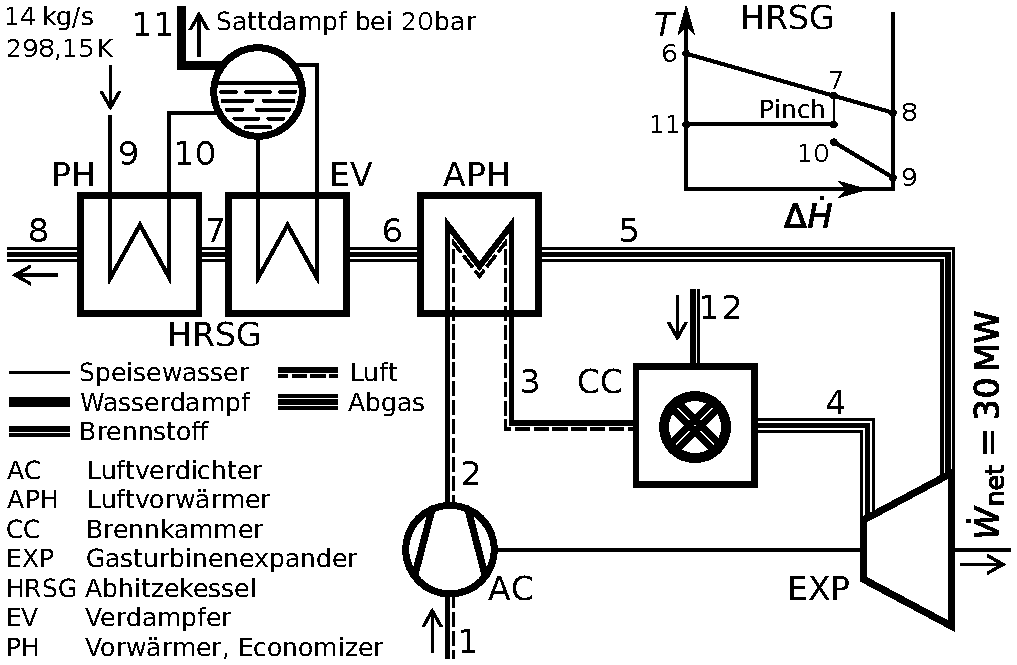
\includegraphics[scale=0.5875]{bilder/cgam-komplett.pdf}		
	\end{center}
}

\headerbox{Vorgaben}{name=vorgaben,column=1,below=einleitung,span=1}{
Die Tabelle fasst relevante vorgegebene Größen zusammen.

	\begin{center}
	\label{tab:vorgaben}
	\begin{tabular}{lllc}
			\toprule
			Parameter & Symbol & Einheit & Wert \\
			\midrule
			Umgebungstemperatur & $T_0$ & \si{\celsius} & 25 \\
			Umgebungsdruck & $p_0$ & \si{\bar} & 1 \\
			Nettoleistung & $\dot W_\text{netto}$ & \si{MW} & 30 \\
			Massenstrom, Dampf & $\dot m_9$ & \si{kg/s} & 14 \\
			Druck des Sattdampfes & $p_{11}$ & \si{bar} & 20 \\
			\bottomrule    
	\end{tabular}
    \end{center}

Wichtige Annahmen und Vereinfachungen:

\begin{compactitem}
    \item Stationärer Prozess
    \item Alle Komponenten nach außen adiabat
    \item Druckverluste vernachlässigt
    \item Gute Laune!
    \item Gruppenarbeit macht Spaß.
\end{compactitem}
}

\headerbox{Ebsilon}{name=ebsilon,column=0,below=fliessbild,span=1}{
Ebsilon toll. Oberfläche toll. Implementierung toll.

Punkte, die beim Modellieren und Simulieren nicht so toll sind:

\begin{compactitem}
    \item kein mp3-plugin
    \item keine automatische Modellerstellung
    \item \dots
    \item jetzt fällt mir nix mehr ein. 
\end{compactitem}
}

\headerbox{TESPy}{name=tespy,column=1,below=fliessbild,span=1}{
TESPy noch toller. Oberfläche schöner. Implementierung super.

Punkte, die beim Modellieren und Simulieren nicht so toll sind:

\begin{compactitem}
    \item auch kein mp3-plugin
    \item auch keine automatische Modellerstellung
    \item \dots
    \item aber sonst alles gut.
\end{compactitem}
}

\headerbox{Auswertung -- Diagramm}{name=diagramm,column=0,below=ebsilon,span=1}{
	\begin{center}
		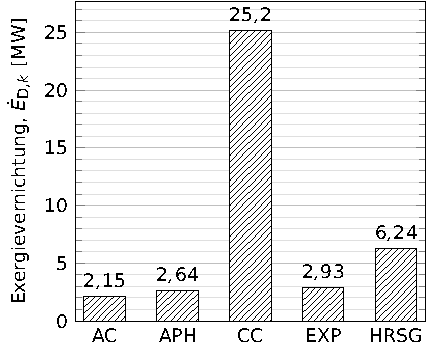
\includegraphics[scale=0.95]{bilder/cgam-diagramm.pdf}		
	\end{center}
}

\headerbox{Auswertung -- Tabelle}{name=tabelle,column=1,below=ebsilon,span=1}{

Alle Ergebnisse für die Ströme stammen aus der Simulation mit TESPy. Die Abweichung der Ergebnisse bei der physikalischen Exergie sind gemäß der folgenden Gleichung angegeben. 
\begin{equation}
\Delta e^\text{PH}=e_\text{TESPy}^\text{PH}-e_\text{Ebsilon}^\text{PH}
\end{equation}
	
	\begin{center}
	\label{tab:auswertung}
	\begin{tabular}{lccccc}
			\toprule
			Strom $j$ & $\dot m_j$ & $p_j$ & $T_j$ & $e_j^\text{PH}$&$\Delta e^\text{PH}$ \\
			&kg/s&bar&\si{\celsius}&kJ/kg&kJ/kg\\
			\midrule
			1&&&&&\\
			2&&&&&\\
			3&&&&&\\
			4&&&&&\\
		
			\bottomrule    
	\end{tabular}
    \end{center}
}


\headerbox{Vergleich}{name=vergleich,column=0,below=diagramm,span=2}{
Gleichung:

\begin{equation}
\sum_i{\left(c_i\dot E_i\right)_k} + \underbrace{\frac{\left(CC_\ell+OMC_\ell\right) BMC_k}{\tau \sum_k{BMC_k}}}_{\dot Z_k=\dot Z_k^\text{CI}+\dot Z_k^\text{OM}}
=\sum_e{\left(c_e\dot E_e\right)_k} + c_{\text{w,}k} \dot W_k + c_{\text{q,}k}\dot E_{\text{q,}k}
\label{eq:cost_balance}
\end{equation}

Chemische Formel:

\begin{equation}
\ce{2NaCl + 2H2O -> 2NaOH + Cl2 + H2}
\end{equation}
}

\headerbox{Ergebnis, Fazit}{name=ergebnis,column=0,below=vergleich,span=1}{
Das haben wir herausgefunden. Das ist wichtig:
\begin{compactitem}
	\item erster Punkt
	\item zweiter Punkt
	\item dritter Punkt
	\item ...
\end{compactitem}
}

\headerbox{Literatur}{name=literatur,column=1,below=vergleich,span=1}{
\AtNextBibliography{\footnotesize}
\setlength\bibitemsep{0pt}
\printbibliography[heading=none]
}

\end{poster}
\end{document}